\documentclass[memoire.tex]{subfiles}
\begin{document}
\chapter{Implémentation}

\subsection{Objectifs}

Notre but étant de pouvoir proposer aux étudiants de première année les éventuelles voix qu'ils sont susceptibles de poursuivre tout au long de leurs études. Le premier objectif de cette étude est dans un premier temps de pouvoir trier les cursus des étudiants précédents en fonction des filières que ceux-ci ont suivies. Cette première phase de catégorisation nous permettra par la suite de conditionner l'algorithme utilisé. Cependant, la réelle problématique est que pour un CV donné, il sera nécessaire de prendre en considération chaque ligne du parcours d'un ancien étudiant comme une occurrence unique et trouver une méthode permettant de représenter graphiquement l'ensemble de celles-ci afin de pouvoir représenter un parcours professionnel.

\subsection{Méthode proposée}

\subsubsection{Le jeu de données}

Pour cette étude, le jeu de données utilisé contiendra environ 2000 CV  d'un projet pouvant être trouvé à l'adresse suivante : \begin{itemize}
\item \url{https://github.com/JAIJANYANI/Automated-Resume-Screening-System}
\end{itemize}
Un premier tri a été effectué afin de filtrer les documents en fonction du format utiliser afin de ne retenir que ceux au format \textbf{.doc} ou \textbf{.docx} pour faciliter les traitements visant ensuite à les classifier. En outre, ce premier tri permettra par la suite de minimiser la charge de calcul afin que les étapes de traitement et d'analyse ne soient pas impactées par un temps de traitement trop important. À noter que bien que cette première étape de tri aurait pu être réalisée de façon manuelle, l'objectif final étant de proposer cette solution sous la forme d'un programme, il est plus intéressant que cette phase de tri puisse s'effectuer de façon automatique une fois le jeu de données fourni.

\newpage
\subsubsection{Choix de l'algorithme}
Afin de pouvoir choisir l'algorithme le plus adapté à notre cas, celui-ci doit pouvoir répondre aux critères suivant : \begin{itemize}
\item Capacité à traiter des documents
\item Capacité à gérer une montée en charge
\item Consommation de mémoire 
\end{itemize}
Comme vu précédemment, l'algorithme K-means bien que celui-ci puisse traiter des documents texte, il impose toutefois de connaitre le nombre de clusters souhaités afin de pouvoir effectuer son traitement.\\
Dans notre cas, cette contrainte ne représente pas de difficultés les CV étant regroupés en fonction des secteurs d’activités (figure à voir). En outre, l’algorithme choisi étant utilisé à travers la librairie python « scikit-learn », celle-ci propose un tableau comparatif (figure 2.1)  des différents algorithmes qu’il est possible d’implémenter en plus de DBSCAN et Agglomerative clustering.
	\begin{figure}[h!]
		\centerline{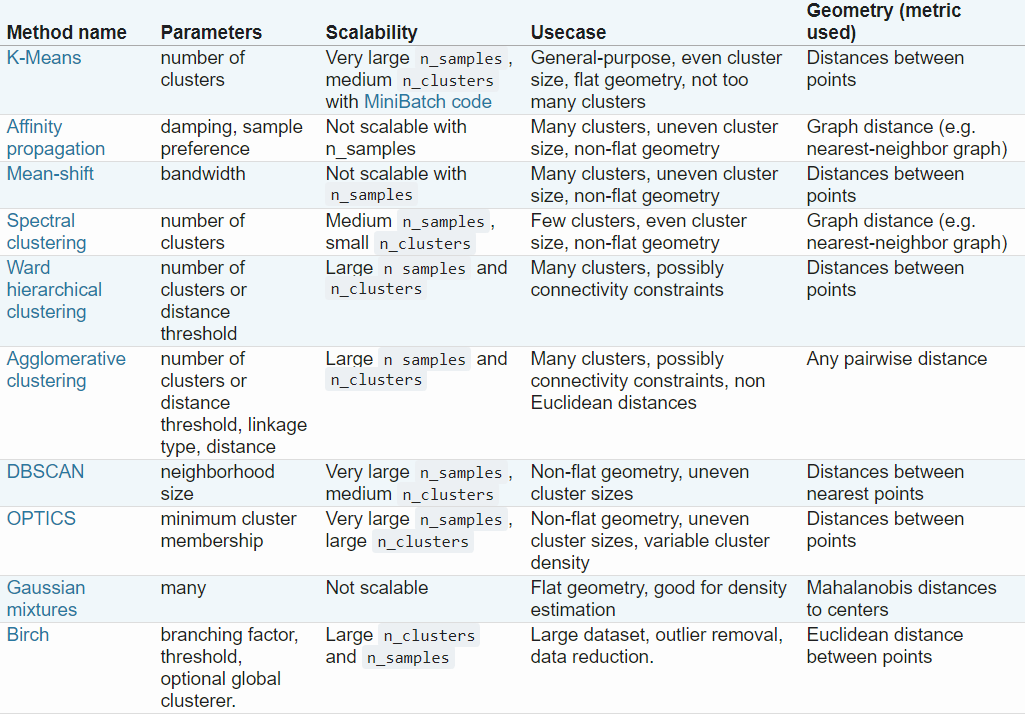
\includegraphics[scale=0.6]{img/algo_table.png}}
		\caption{Comparatif des algorithmes de clustering}
	\end{figure}
Au vu des différents cas d’utilisation proposés par ce tableau, les trois algorithmes étudiés dans ce document peuvent être implémentés. K-means étant le plus courant et possédant une facilité d’implémentation sera l’algorithme utilisé étant donné qu’il est également possible de l’utiliser dans le traitement de documents. La représentation des données choisie n'est pas adaptée à l'utilisation de DBSCAN. De plus, nous sommes dans un cas d'apprentissage non supervisé, cet algorithme nécessite une configuration établie en amont par un utilisateur. En revanche,K-means bien qu'ayant besoin du nombre de clusters souhaités peut fonctionner sans que des labels lui soit fourni.
\subsection{Démarche}
Afin de pouvoir utiliser l'algorithme K-Means, il est nécessaire dans un premier temps de transformer notre base de données en un format interprétable par notre/nos algorithmes. Afin de pouvoir fonctionner, K-means utilise des données numériques sous la forme illustrée la figure 2.2 par conséquent, grâce à la structure des dossiers ou sont stockés, il est possible de créer une énumération afin de pouvoir attribuer une valeur aux différentes catégories, de plus cette structure nous permet de déterminer le K maximum qu’il est possible d’adopter pour les différentes opérations de l’algorithme. Une fois cette énumération créée, celle-ci nous permet donc de catégoriser les différents CV en fonction du secteur auquel ceux-ci sont le plus fortement liés.
	\begin{figure}[h!]
		\centerline{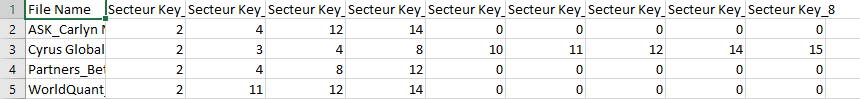
\includegraphics[scale=0.7]{img/data_sample.png}}
		\caption{Extrait du jeu de données}
	\end{figure}

Comme illustrée dans la figure ci-dessus, chaque mot clé correspondant à un secteur d'activité est renseigné dans l'ordre ou ceux-ci sont rencontré durant le traitement de l'algorithme, ce qui permet d'avoir un premier aperçu des filières parcourues par un individu. À noter que la valeur 0 sert à représenter un vide afin que le jeu de données puisse être interprété par K-means.\\
Une fois cette première étape exécutée, il est alors possible d'utiliser K-means pour la création de nos clusters. Dans notre cas, nous avons tenté de lancer l'algorithme sans lui fournir de labels au préalable afin de pouvoir mesurer son taux de précision.(figure 2.3)
	\begin{figure}[h!]
		\centerline{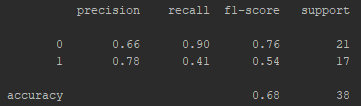
\includegraphics[scale=0.7]{img/result_kmeans.png}}
		\caption{Résultat de création de clusters par K-means}
	\end{figure}
Dans cet exemple, nous avons créé un cluster contenant tous les CV dont le propriétaire a commencé par une filière administrative. On peut observer un taux de 78\% de réussir dans la détermination de l'appartenance à la filière recherchée sans aucun apport de la part de l'utilisateur.
\subsection{Problématiques restantes}
Nous avons pu voir qu’il existe une multitude de méthodes applicables afin d’ordonner nos données, cependant la première problématique rencontrée pour cette implémentation a été le parsing des CV. Il est en effet possible de récupérer aisément les mots clés recherchés tels que « Sales » ou encore « Law » comme filière universitaire ou secteur d’activité professionnelle. La difficulté vient toutefois du fait qu’il est nécessaire de différencier dans quelle rubrique du CV, dans notre cas « Education » ou « Work experience » ces mots apparaissent. Ce type de découpage de document est en général utilisé par les services de recrutement d’entreprise lorsqu’un recruteur cherche un profil en fonction de mots clés ce qui fait que ces solutions sont propriétaires. Un projet open source disponible à l’adresse suivante :
\begin{itemize}
\item \url{https://github.com/tramyardg/CVparser}
\end{itemize}

Ce projet aurait pu représenter une solution possible. Celui-ci renvoie une chaine de caractère au format JSON contenant les différentes rubriques découpées. Malencontreusement, ce projet n’est plus fonctionnel ni maintenu par son créateur.
La seconde problématique restante vient du fait que pour notre cas d’étude, une fois les différents parcours universitaires ainsi que le secteur occupé ont été classifiés, afin de pouvoir modéliser ces trajectoires sous forme graphique, il serait nécessaire de pouvoir récupérer le contenu d’un objet lui-même contenu dans un cluster donné et pouvoir considérer chaque ligne comme un objet unique afin de pouvoir modéliser celle-ci sous forme de point. Cette seconde problématique est par conséquent fortement liée à la première de par le fait qu’il est nécessaire dans un premier temps de pouvoir traiter les différentes rubriques d’un document une à une et d’être en mesure de ne récupérer que des données pertinentes.

\subsection{Conclusion}
Dans ce mémoire, nous avons présenté les différentes méthodes de clustering, dont le clustering par partitionnement qui semble correspondre à notre cas. Toutefois, le clustering hiérarchique reste prometteur. Cependant le traitement des objets clusterisés et le découpage de document ont entrainé la rencontre de nouvelle problématique durant cette étude.\\
L'analyse de données étant un élément essentiel de domaine qui de nos jours possède une forte popularité tel que le Big data. Les méthodes de clustering utilisées dans ce domaine représentent une opportunité prometteuse pour notre problématique. En effet, celles-ci nous permettent dans un premier temps d'ordonner nos données afin de pouvoir en dégager les populations principales. Cette première étape de classification et représentation des données permet ensuite de faciliter les différents traitements.\\
Dans la dernière partie, nous avons présenté la première partie d'une méthode visant à tirer profit de la classification obtenue à travers des processus de clustering. Plus particulièrement, nous avons eu recours à un clustering par partitionnement afin de pouvoir identifier les différentes populations. De plus, le type de cluster utilisé est "well-separated", ce qui nous évite d'avoir des objets pouvant se trouver dans plusieurs clusters. Cependant, cette méthode pose de nouvelles problématiques dans le cas de parcours contenant plusieurs filières et n'est par conséquent pas la plus idéale.Toutefois, il reste encore une partie conséquente de l'implémentation regardant l'extraction de texte à réaliser.
\end{document}

